\section{Discussion}
\label{sec:discussion}

\paragraph{When is simplification safe?}
Our results across four evaluation dimensions consistently indicate that
MDL-to-UsdPreviewSurface conversion is safe for assets whose appearance is
dominated by standard PBR channels (diffuse albedo, roughness, metallic,
normal). For such assets, we observe PSNR $>$ 35\,dB, SSIM $>$ 0.99, CLIP
similarity $>$ 0.92, and no systematic change in detection behavior. Caution is
warranted for materials that rely on multi-layer MDL effects --- procedural
noise textures, specular coatings, and anisotropic reflectance --- where
per-viewpoint PSNR can drop below 25\,dB and DINOv2 similarity below 0.60. We
recommend that practitioners validate such materials individually using the
feature-level metrics introduced here, which are more sensitive to perceptually
relevant differences than pixel-level metrics alone.

\paragraph{The within-simulation rendering gap.}
Much prior work has focused on the sim-to-real
gap~\cite{Tobin2017Domain,Tremblay2018Training,Zhao2020Sim,Garcia2023Robust}:
the distribution shift between synthetic and real images. Our work highlights a
complementary and less-studied phenomenon --- the \emph{within-simulation
rendering gap} --- arising from differences in material representation within
the same renderer. When converting MDL to UsdPreviewSurface, geometry, lighting,
and camera parameters remain identical; only the material shader changes. The
resulting image differences are therefore a pure measure of how much visual
information is lost when reducing a high-fidelity material model to a simpler
one. Our finding that this gap is small (SSIM $>$ 0.99, CLIP $>$ 0.92) for
standard PBR assets leads us to hypothesize that, for many practical
applications, the within-simulation gap introduced by material simplification
is small relative to typical sim-to-real gaps reported in the literature.

\paragraph{Interoperability versus fidelity.}
The primary motivation for material simplification is not rendering performance
--- which we show is effectively unchanged for single-object scenes --- but
interoperability. UsdPreviewSurface materials are supported by standard USD
viewers, web-based 3D platforms, and the glTF/GLB export path, none of which
can interpret NVIDIA's proprietary MDL shaders. Our results quantify the cost
of this interoperability gain: a mean LPIPS increase of 0.020 and a DINOv2
cosine similarity of 0.872. For synthetic data pipelines where downstream
models operate on features rather than pixels, this trade-off is favorable.

\paragraph{Why DINOv2 is more sensitive than CLIP.}
Figure~\ref{fig:tsne_dino} provides a t-SNE visualization of DINOv2 embeddings
for all 48 rendered images. MDL and UsdPreviewSurface renderings of the same
scene cluster tightly together, confirming that material simplification produces
a smaller feature-space perturbation than the inter-scene variation.

\begin{figure}[t]
\centering
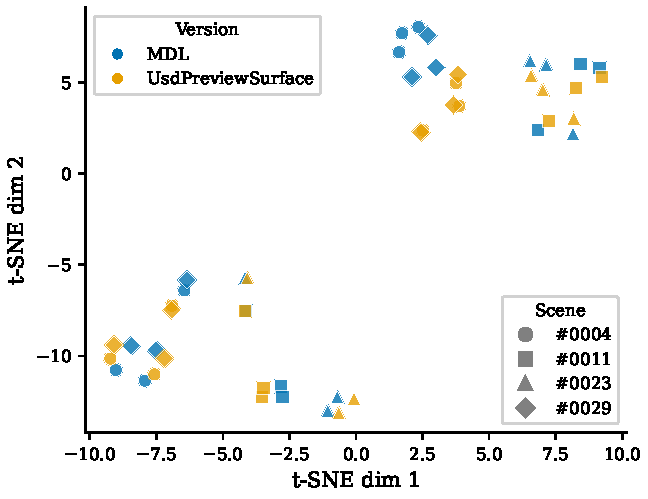
\includegraphics[width=\linewidth]{../results/figures/fig_tsne_dino.pdf}
\caption{t-SNE projection of DINOv2 ViT-B/14 embeddings for all 48 images
(24 MDL + 24 UsdPreviewSurface), computed with perplexity\,=\,12,
learning rate\,=\,auto, and PCA initialization (random seed\,=\,42).
Same-scene pairs cluster tightly, indicating that the within-material
perturbation is small relative to inter-scene variation in the DINOv2
feature space.}
\label{fig:tsne_dino}
\end{figure}

CLIP's contrastive language--image pre-training~\cite{Radford2021Learning}
optimizes for high-level semantic alignment between images and text, producing
representations that are naturally invariant to low-level appearance changes
such as texture detail, specular highlights, and subtle color shifts. DINOv2's
self-supervised objective~\cite{Oquab2023DINOv2}, by contrast, preserves
fine-grained spatial and textural features, making it more sensitive to exactly
the kind of local appearance differences that material simplification
introduces. The gap between CLIP (0.925) and DINOv2 (0.872) similarity thus
reflects the granularity of each model's learned representations rather than a
deficiency in the conversion. Practitioners should select the appropriate
metric based on their downstream task: CLIP similarity is most relevant for
tasks relying on high-level semantics (e.g., image--text retrieval,
classification), while DINOv2 similarity better captures texture-level fidelity
relevant to dense prediction tasks (e.g., segmentation, depth estimation).

\paragraph{Interpreting sparse detection results.}
The low absolute detection rate in our zero-shot experiment (4--7 of 24 images
per version) is a consequence of the evaluation design: single-object renders
on plain backgrounds fall far outside YOLOv8's COCO training
distribution~\cite{Jocher2023YOLO}. While the small number of detections limits statistical power, we observe no
systematic difference in which viewpoints trigger detections or in their
associated confidence scores. This preliminary observation suggests that
material simplification does not introduce obvious artifacts that confuse
pre-trained detectors, though confirmation with larger sample sizes is needed.
Future work should evaluate with detectors fine-tuned on synthetic data, where
the material representation directly influences training signal quality.

\paragraph{Practical recommendations.}
Based on our findings, we offer the following guidelines for synthetic data
practitioners working with Isaac Sim assets:
\begin{enumerate}
    \item \textbf{Default to conversion} for assets with standard PBR materials.
    The quality loss is negligible and the interoperability benefits are
    significant.
    \item \textbf{Validate complex materials} using CLIP and DINOv2 cosine
    similarity as quick diagnostic metrics before deploying converted assets in
    training pipelines.
    \item \textbf{Use CLIP similarity as a go/no-go threshold.} A per-pair CLIP
    cosine similarity below 0.85 may indicate material features that are poorly
    captured by UsdPreviewSurface and warrant manual inspection. In our
    experiments, one pair falls below this threshold, corresponding to a
    viewpoint with complex specular effects.
    \item \textbf{Monitor DINOv2 for texture-sensitive tasks.} If the downstream
    task depends on fine-grained texture features, require DINOv2 similarity
    above 0.80 as an additional quality gate. In our experiments, three pairs
    fall below this threshold, all corresponding to viewpoints with complex
    specular effects.
\end{enumerate}
We note that these guidelines are derived from furniture assets with
predominantly wood, metal, and fabric materials; validation on diverse object
categories (e.g., transparent, organic, or highly specular surfaces) is needed
before broader generalization.
